\chapter{Introducción}

    Los números aleatorios se utilizan en muchos ámbitos de la vida cotidiana. Se utilizan para elegir quién gana la lotería, para determinar quién ataca primero en un partido de fútbol, para garantizar una partida justa en juegos de mesa y desempeñan un papel fundamental en la criptografía y la seguridad de la información. Para seleccionar al equipo atacante en un partido de fútbol, basta con lanzar una moneda. Sin embargo, para jugar a un juego de mesa se requieren más de dos valores aleatorios, por lo que se utiliza un dado. En cambio, la criptografía requiere algo más que tirar un dado para asegurar la protección de los datos en comunicaciones digitales o en transacciones bancarias. La seguridad de las comunicaciones es una parte fundamental de la vida moderna, en la que las personas envían correos electrónicos, realizan llamadas o envían mensajes a sus amigos y realiza transacciones en línea millones de veces al día. La sociedad confía que cada uno de estos procesos cotidianos sean seguros y confidenciales. La seguridad de las comunicaciones dependen de la capacidad de estos procesos para verificar la identidad de las personas que se comunican. La única forma de garantizar la seguridad es mediante la distribución de identidades privadas conocidas solo por el usuario, denominadas claves. Las claves privadas son números aleatorios únicos generados para cada usuario, que aseguran que personas malintencionadas no puedan suplantar a nadie y causar daño. La aleatoriedad de los números de las claves privadas es crucial para garantizar la seguridad de las conexiones. La capacidad de generar números aleatorios es, por tanto, una parte muy importante de la seguridad de los sistemas de comunicación.

    Los números aleatorios tienen una amplia variedad de aplicaciones. Se utilizan en simulaciones a computadora de fenómenos naturales, como en el modelado de la colisión de partículas en física nuclear y en el análisis logístico de pasajeros en aeropuertos en investigación operativa. También son útiles en el muestreo estadístico cuando no es práctico analizar todos los casos posibles. Los números aleatorios son una buena fuente de datos para probar la efectividad de los algoritmos de computadora y son cruciales para el funcionamiento de los algoritmos aleatorios. Además, se utilizan en análisis numérico y en la estética, donde agregar un poco de aleatoriedad hace que los gráficos generados por computadora y la música parezcan más vivos. En algunos casos, es importante tomar decisiones completamente imparciales y la aleatoriedad es esencial en las estrategias óptimas de la teoría de juegos. Ejecutivos y profesores universitarios recurren a estas estrategias con frecuencia, tirando una moneda o lanzando dardos \cite{Knuth2014}. 

    En un sistema criptográfico, se utilizan generadores de números aleatorios o Random Number Generators (RNG), no sólo para generar claves criptográficas, sino también para generar números de un solo uso (nonces), valores de relleno, vectores de inicialización, desafíos y máscaras aleatorias para la protección contra ataques de canal lateral \cite{Petura2016}.

    A pesar de que hay muchas aplicaciones diferentes de los números aleatorios, todos comparten dos requisitos básicos: buenas propiedades estadísticas, concretamente una distribución de probabilidad uniforme donde cada valor de cualquier número aleatorio tenga la misma probabilidad de aparecer, e imprevisibilidad de los números aleatorios. Los números aleatorios, especialmente los utilizados para parámetros secretos como las claves, deben ser impredecibles para evitar que un atacante pueda calcular valores futuros o anteriores a partir de los datos ya generados y capturados. En los diseños modernos, se requieren algunas características adicionales: el generador debe ser intrínsecamente seguro, robusto y resistente a los ataques y probado en línea mediante pruebas específicas del generador \cite{Badrignans2011}. Los números aleatorios son una herramienta valiosa y versátil que se utiliza en prácticamente todos los ámbitos de la ciencia y la tecnología y su importancia en la seguridad es fundamental.

    En 1999, Intel introdujo el generador de números aleatorios basado en silicio \cite{Jun1999}, ese RNG fue el primero de la familia de primitivos de Intel, lanzado para la protección de datos y comunicaciones dentro del hardware del PC. Desde ese entonces muchos científicos han buscado la manera de crear mejores sistemas integrados que generen números aleatorios para proteger los datos de los usuarios. En este esfuerzo se ha desarrollado toda una metodología para analizar, categorizar y evaluar los RNGs. Agencias de estandarización como la NIST (National Institute of Standards and Technology) \cite{Turan2018} en Estados Unidos o la BSI (Federal Office for Information Security) \cite{AIS2011} en Alemania han creado una serie documentaciones, recomendaciones y pruebas estadísticas para evaluar los generadores de números aleatorios.

 \section{Clasificación de los RNGs}

        Dado el amplio rango de aplicaciones de los RNG, existen diferentes clases de RNG que satisfacen diversas necesidades. Basándonos en el método utilizado para generar números aleatorios, podemos distinguir dos tipos fundamentales de RNG:
	        
        \begin{enumerate}
            \item Generadores de números aleatorios deterministas (DRNG/PRNG)
            
                También conocidos como generadores de números pseudo-aleatorios o Pseudo-Random Number Generators (PRNG), son sistemas que producen una secuencia de aspecto aleatorio de forma matemática, es decir, hay un algoritmo subyacente y debido a esto los Deterministic Random Number Generators (DRNG) son fáciles de implementar en dispositivos lógicos. Si se conoce el algoritmo, la salida del generador es predecible. Incluso cuando no se conoce el algoritmo pero se han guardado algunas de las secuencias de salida del generador, su comportamiento durante la secuencia guardada puede utilizarse en futuros ataques. Los números producidos parecen aleatorios a corto plazo, pero la secuencia es periódica, normalmente con un periodo largo. Para producir una salida menos predecible, estos generadores utilizan valores de inicialización llamados semillas para empezar a generar números \cite{Nist2010}. Para cada semilla se genera una secuencia diferente. Por esta razón, los DRNG deben ser computacionalmente seguros, el algoritmo no debe poder adivinarse computacionalmente y su valor inicial nunca debe reutilizarse. La reutilización del valor inicial puede evitarse guardando el último valor haciendo uso de un contador y utilizando el siguiente valor del contador la próxima vez. La secuencia de salida de un buen DRNG está perfectamente distribuida de manera uniforme, en otras palabras, tienen buenas propiedades estadísticas. Además, los DRNGs consiguen altas tasas de bits de salida y suelen utilizarse como generadores de claves en los cifrados de flujo \cite{Badrignans2011}.
            
            \item Generadores de números aleatorios verdaderos (TRNG)
            
                Los True Random Number Generators (TRNG) son sistemas que extraen la aleatoriedad de fenómenos aleatorios no algorítmicos impredecibles como fluctuaciones de temperatura, decaimiento radiactivo, ruido de radio ambiental, tiempos de acceso al disco duro o interacciones del usuario con el PC, jitter, entre otros. A diferencia de los DRNG, que utilizan fórmulas matemáticas para generar números aleatorios, los TRNG producen datos aleatorios reales que no se pueden predecir. Sin embargo, debido a que los procesos físicos utilizados por los TRNG están sujetos a fluctuaciones, la calidad de la secuencia aleatoria generada puede presentar algunos defectos estadísticos, como el sesgo.
                
                Dado que los procesos físicos están sujetos a fluctuaciones, las características estadísticas de los TRNG suelen ser peores que las de los DRNG y están estrechamente relacionadas con la calidad de la fuente de entropía y con el método de extracción de la aleatoriedad. La velocidad final de los TRNG está limitada por el espectro de la señal aleatoria y por el principio utilizado para extraer la entropía de la misma, por ejemplo, la frecuencia de muestreo vinculada al espectro del ruido. En general, los TRNG son, más lentos que los DRNG. Dependiendo de la fuente utilizada los TRNG se pueden dividir en:
            
            \begin{itemize}
                \item Físicos (PTRNG), utilizan ruido físico a nivel de electrones presente en todos los semiconductores. Es un dispositivo físico y utiliza ruido físico.
                \item No físicos (NPTRNG), pueden no ser dispositivos físicos, sino más bien una pieza de software que utilizan fuentes de aleatoriedad no físicas, como las interacciones del usuario con un sistema operativo, por mencionar algunas el movimiento del cursor del mouse.
            \end{itemize}
        \end{enumerate}
	
        La imprevisibilidad de los generadores de números aleatorios deterministas está garantizada computacionalmente, mientras que la imprevisibilidad de los generadores verdaderamente aleatorios está garantizada por fenómenos físicos aleatorios y se caracteriza por la tasa de entropía a la salida del generador. Tanto los TRNG como los DRNG tienen sus ventajas y desventajas, por lo que muchos sistemas criptográficos utilizan RNG híbridos. Los generadores de números aleatorios híbridos, conocidos como Hybrid Random Number Generators (HRNG) combinan las fortalezas de los DRNG (rápidos y de buena calidad) sembrados repetidamente por un TRNG (lento pero impredecible). Es importante encontrar un equilibrio entre la velocidad del generador y su imprevisibilidad ajustando el intervalo de tiempo entre semillas y el tamaño de la semilla. En función de su implementación, existen dos tipos de RNG híbridos:
	
        \begin{enumerate}		
            \item Generadores de números aleatorios verdaderos híbridos
            
            Combinan un TRNG con un postprocesamiento criptográfico. El postprocesamiento criptográfico asegura el secreto hacia adelante y hacia atrás de los números aleatorios producidos, no pueden calcularse los valores pasados o los futuros a partir del valor actual. Si la fuente física falla, también garantiza unas propiedades estadísticas perfectas de los datos de salida, ya que el núcleo de un postprocesamiento criptográfico suele ser un cifrador. La tasa de bits de salida de un TRNG híbrido está limitada por la del núcleo del TRNG.
            
            \item Generadores de números aleatorios deterministas híbridos. 
            
                Utilizan un TRNG para generar periódicamente semillas para un DRNG. Dado que la salida de un DRNG es predecible si conocemos su semilla, ir renovando la semilla mediante un TRNG puede reducir la predictibilidad de un DRNG híbrido. Además la secuencia de salida de un generador de este tipo es perfectamente uniforme, lo que podría no ser el caso de un TRNG puro. Su tasa de bits de salida viene determinada por la tasa de bits del DRNG subyacente, ya que se pueden producir números aleatorios mientras no se alcance el periodo de repetición del DRNG.
        \end{enumerate}

        Para garantizar la seguridad de las claves confidenciales, es fundamental que se generen dentro del sistema criptográfico. Dado que la mayoría de los sistemas criptográficos actuales se implementan en dispositivos lógicos y sistemas digitales utilizando algoritmos y protocolos criptográficos, es natural que la investigación se centre en la implementación de generadores de números aleatorios en dispositivos lógicos, como los Field-Programmable Gate Arrays (FPGA). Esto ayuda a prevenir el acceso no autorizado a las claves y garantiza que sean generadas de manera segura y confiable dentro del sistema criptográfico.
    
        A pesar de la menor velocidad de los TRNG, estos se utilizan con más frecuencia en aplicaciones criptográficas que los DRNG. Los TRNG son las únicas primitivas criptográficas que no han sido objeto de normalización hasta ahora. Sin embargo, antes de utilizar un generador en la práctica, el principio de funcionamiento y su implementación dentro de un módulo criptográfico deben ser validados por una institución acreditada como parte de un proceso de evaluación de seguridad. Los generadores que no tienen un certificado de seguridad se consideran inseguros en cuanto a su uso en aplicaciones criptográficas. Por este motivo, es de gran interés el estudio de los principales TRNG existentes y sus características.

	\section{Estructura de los TRNG}	

        La estructura general de un TRNG se muestra en la Figura \ref{fig:A1_TRNG_estructura}. El generador debe utilizar un proceso físico incontrolable como fuente de aleatoriedad. Dado que los fenómenos físicos utilizados en los TRNG son en su mayoría procesos analógicos, suele ser necesario algún método que permita la conversión de datos del dominio analógico al digital. Se puede incluir una conversión de analógico a digital en el procedimiento de extracción de aleatoriedad. La señal binaria sin procesar obtenida, el llamado ruido digital, puede tener baja entropía, malas propiedades estadísticas o ambas. En este caso, se pueden usar algunos algoritmos de postprocesamiento para mejorar los parámetros estadísticos del flujo de bits de salida. Sin embargo, el postprocesamiento de la salida del TRNG a veces puede enmascarar una falla grave en el generador. Las pruebas estadísticas estándar pueden entonces fallar en detectar la debilidad enmascarada. Por lo tanto, se recomienda tener la posibilidad de probar el ruido digital sin procesar o Raw Bit Signal (RBS). La seguridad del generador se puede aumentar si las pruebas estadísticas se aplican sobre la marcha y si están diseñadas para adaptarse al principio de funcionamiento del generador teniendo presente sus posibles debilidades \cite{Badrignans2011}.
			
        \begin{figure}[hbtp]
            \centering
            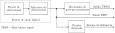
\includegraphics[width=0.9\textwidth]{A0_TRNG_estructura}
            \caption{Estructura general de un TRNG \cite{Badrignans2011}.}
            \label{fig:A1_TRNG_estructura}
        \end{figure}
	
        Los TRNG emplean diferentes fuentes de aleatoriedad y una gran variedad de principios para extraerla. En este sentido, resulta relevante evaluar los principales principios utilizados por los TRNG: parámetros relacionados con la calidad, parámetros relacionados con la seguridad y parámetros relacionados con el diseño.

        \begin{itemize}[noitemsep]
            \item Parámetros relacionados con la calidad
                \begin{itemize}[noitemsep]
                    \item Fuente de aleatoriedad.
                    \item Método de extracción de aleatoriedad y entropía del ruido digital.
                    \item Método de procesamiento posterior aplicado (opcional).
                    \item Tasa de bits de salida y su estabilidad.
                \end{itemize}
            \item Parámetros relacionados con la seguridad
                \begin{itemize}[noitemsep]
                    \item Existencia de un modelo matemático.
                    \item Comprobabilidad interna.
                    \item Seguridad (robustez, resistencia contra ataques).
                \end{itemize}
            \item Parámetros relacionados con el diseño
                \begin{itemize}[noitemsep]
                    \item El uso de recursos.
                    \item El consumo de energía.
                    \item Viabilidad en dispositivos lógicos y FPGAs.
                    \item Automatización del diseño.
                \end{itemize}
        \end{itemize}

        Es fundamental tener en cuenta que no todas las características de los TRNG tienen la misma relevancia en su evaluación. En particular, los parámetros relacionados con la seguridad, tales como la robustez, la disponibilidad de un modelo estocástico y la capacidad de prueba, adquieren una importancia crucial en un sistema de seguridad de datos. Su peso en la evaluación de un TRNG es significativamente mayor que el de otros parámetros, como el consumo de energía o la tasa de bits \cite{Badrignans2011}.

    \section{Condiciones de funcionamiento y calidad de la salida del TRNG}

            Para que un TRNG sea considerado de buena calidad, su salida debe ser prácticamente indistinguible de la salida de un TRNG ideal en todas las condiciones de funcionamiento y a lo largo del tiempo. En el diseño de un TRNG, es fundamental prestar atención tanto a la calidad del flujo de bits generado como a sus parámetros de seguridad, incluyendo la robustez ante el envejecimiento, cambios ambientales, posibles ataques y la existencia de pruebas de autodiagnóstico y en línea \cite{Schindler2003}.
            Un buen TRNG debe proporcionar un flujo de 0s y 1s distribuido uniformemente en su salida. La calidad del flujo de bits generado está estrechamente relacionada con la calidad de la fuente de aleatoriedad y el método utilizado para extraer la aleatoriedad. Las características espectrales de la fuente y el método de extracción determinan los principales parámetros del flujo de bits generado, como el sesgo de los bits de salida, la correlación entre bits sucesivos y patrones visibles. Aunque algunos de estos problemas pueden corregirse mediante un postprocesamiento efectivo, es preferible que el generador produzca intrínsecamente un flujo de bits en bruto de alta calidad.

            Si el extractor muestrea la fuente de aleatoriedad demasiado rápido, los bits adyacentes pueden estar correlacionados. Por esta razón, es una buena práctica comprobar si el flujo de bits generado presenta autocorrelación a corto plazo. Además, pueden existir otras dependencias a corto plazo en el ruido digital, que deben detectarse mediante pruebas específicas del generador. El comportamiento del generador puede verse afectado por interferencias eléctricas externas e internas. Un efecto evidente de estas interferencias son las frecuencias discretas que se originan en la fuente de alimentación y en diversas señales internas que aparecen en el espectro de ruido.

            La señal de ruido generada puede verse significativamente afectada por el ruido de baja frecuencia causado por los semiconductores. Además, las capacidades internas pueden involuntariamente filtrar las frecuencias altas del espectro de ruido. Algunos generadores pueden presentar lo que se conoce como puntos malos, que son breves periodos en los que el generador deja de funcionar debido a interferencias eléctricas o sobrecargas en la parte sobrecargada del circuito.

            Una característica peligrosa del generador es la existencia de una puerta trasera, que se refiere a las desviaciones de la aleatoriedad uniforme introducidas deliberadamente por el fabricante. Por ejemplo, supongamos que en lugar de utilizar un proceso físico, el generador genera una secuencia pseudoaleatoria de alta calidad con una semilla de 40 bits. Aunque sería imposible detectar este comportamiento aplicando pruebas estadísticas estándar al flujo de bits de salida, alguien que conozca la puerta trasera podría adivinar las claves sucesivas mediante un proceso computacionalmente factible. 


    En este trabajo nos enfocaremos en los generadores que pueden implementarse en sistemas digitales y en específico en FPGAs. 

    \section{Trabajos actuales}

        Desde hace una década los TRNGs implementados en FPGA han ido evolucionando y fue en 2016 cuando \cite{Petura2016} hizo una recopilación de todos los núcleos TRNGs que cumplen con las características descritas por la AIS20/31. Los TRNG destinados a ser utilizados en aplicaciones criptográficas deben cumplir con los siguientes requisitos: 1) su diseño debe ser sencillo y comprensible, la fuente de aleatoriedad debe estar claramente definida; 2) el proceso aleatorio subyacente debe ser estacionario y el modelo estocástico debe ser factible; 3) la señal binaria sin procesar debe estar disponible para posteriores pruebas off-line y on-line. Además, es útil que la fuente de aleatoriedad (por ejemplo, el jitter del reloj procedente del ruido térmico) sea cuantificable: su medición dentro del dispositivo puede servir de base para realizar pruebas estadísticas integradas rápidas y eficaces.

        Además seleccionó núcleos TRNG que utilizan circuitos oscilantes: osciladores en anillo de evento único (es decir, osciladores en anillo estándar) \cite{Baudet2010}, \cite{Kohlbrenner2004}, osciladores en anillo multievento con colisiones de señal (es decir, osciladores en anillo de efecto de transición) \cite{Varchola2010}, osciladores en anillo multievento sin colisiones de señal (es decir, anillos autotemporizados) \cite{Cherkaoui2013} y bucles de fase bloqueada (PLL) \cite{Fischer2003}. Todos ellos deberían ser viables en las familias recientes y futuras de FPGAs. Todos ellos utilizan fuentes de aleatoriedad sencillas y comprensibles, su señal aleatoria sin procesar está disponible fuera del generador, y el modelo estocástico del generador existe o es factible. Por lo tanto, todos ellos cumplen los requisitos de AIS-20/31.

    Con base en los criterios del AIS-20/31, los núcleos TRNG adecuados para utilizarse en dispositivos lógicos programables (FPGA) que usan estructuras oscilantes son:

        \begin{itemize}
            \item Elementary ring oscillator based TRNG (ERO-TRNG).
            \item Coherent sampling ring oscillator based TRNG (COSO-TRNG).
            \item Multi-ring oscillator based TRNG (MURO-TRNG).
            \item Transient effect ring oscillator based TRNG (TERO-TRNG).
            \item Self-timed ring based TRNG  (STR-TRNG).
            \item Phase-locked loop based TRNG (PLL-TRNG).
        \end{itemize}

    En años recientes se ha buscado mejorar estos núcleos haciendo variaciones en las conexiones de los componentes internos sin modificar el método de extracción de aleatoriedad. En \cite{Wang2021} se diseño un TRNG basado en PLLs y su contribución se enfocó en analizar su comportamiento a variaciones de voltaje y temperatura, utilizó 56 LUTs, 19 Registros y obtuvo una velocidad de salida de 100 Mbit/s. En \cite{Peetermans2021} se modificó un TRNG basado en el núcleo COSO utilizando una Xilinx Spartan 7, pasó las pruebas estadísticas AIS-31, las NIST y tuvo una velocidad de salida de 1.47 Mbit/s. En \cite{Anandakumar2020} se diseño un TRNG basado en retardos de osciladores de anillo y posteriormente se realizó un postprocesamiento corrector Von Neumann, pasó todas las pruebas NIST, utiliza 528 slices de una Xilinx Spartan 3-A y obtuvo una velocidad de salida de 6 Mbit/s.

    Los artículos anteriores se enfocan en mejorar los núcleos para obtener mejores tasas de bits de salida, disminuir el uso de recursos o mejorar la robustez, sin embargo, existe otro enfoque que consiste en utilizar los TRNG únicamente para generar la semilla de un DRNG. Es decir, crear TRNGs híbridos que combinen las mejores característica de ambos generadores. Además el uso de caos como postprocesamiento o DRNG ha crecido en los años. En \cite{Liao2022} se discretiza un sistema dinámico caótico y se genera una estructura combinada para sembrar el sistema y obtener números aleatorios, se utilizaron 12383 LUTs, 134883 registros, 145 DSPs de una FPGA de la familia Xilinx. En \cite{Vaidyanathan2021} se utiliza un sistema hipercaótico de 5 dimensiones discretizado utilizando los métodos numéricos de forward Euler, trapezoidal, y Runge-Kutta de cuarto orden para diseñar un TRNG híbrido, obtuvo una velocidad de salida de 416 Mbit/s y utiliza 1648 LUTs y 1112 registros. En \cite{Fraga2017} se estudiaron diversos mapas caóticos para utilizarse como DRNG implementados en FPGA, se analizó cual de todos los mapas estudiados genera los mejores resultados y se concluyó que el mapa de corrimientos de Bernoulli es el mejor, utilizando 575 LUTs, 108 registros y obteniendo  una velocidad de salida de 7.389 Mbit/s. En los artículos anteriores se busca aprovechar el caos para aumentar la tasa de bits de salida de los TRNG, sin embargo esto es a costa de aumentar el uso de recursos. 

    Se ha probado extensamente que el caos es una herramienta muy útil para generar números aleatorios y en particular se utiliza mucho para crear esquemas de cifrado \cite{Wong2008,AlHazaimeh2017,Liu2020}, cifrado de imágenes \cite{Li2013, Sivaraman2020,Pareek2006,Kadir2010,Liu2016,Vaidyanathan2018,GarciaGuerrero2020} y en particular los mapas caóticos han cobrado popularidad debido a que su estructura matemática por lo general es sencilla y puede describirse en hardware utilizando pocos recursos, a diferencia de los sistemas dinámicos caóticos en tiempo continuo los cuales requieren el uso de métodos numéricos y su implementación no es trivial.

    Nuevos mapas caóticos \cite{GarciaGrimaldo2021} con mejores características se han estudiado en recientes años lo que abre la posibilidad de poder seguir mejorando los DRNGs. Además sistemas integrados con co-diseño, FPGA-Soc, \cite{HernandezMorales2022} hacen cada vez más fácil poder realizar las pruebas estadísticas en linea y hacer sistemas cada vez más robustos. 

    En este trabajo utilizaremos un TRNG para sembrar un DRNG basado en un mapa caótico bidimensional, probaremos sus características estadísticas utilizando las pruebas NIST y analizaremos la versatilidad del diseño analizando las variaciones del mapa caótico.


    \section{Objetivos}
	
		\subsection{Objetivo general}
			\begin{itemize}
				\item Diseñar e implementar en FPGA un TRNG híbrido para la generación de secuencias muy largas.
			\end{itemize}
		
		\subsection{Objetivos específicos}
			\begin{itemize}
                \item Investigar el estado del arte de diferentes generadores de números aleatorios.
                \item Estudiar los diferentes tipos de generadores de números aleatorios y analizar sus características principales.
                \item Estudiar la teoría de los mapas caóticos y su utilidad en generadores de números aleatorios.
                \item Diseñar un generador de números aleatorios híbrido utilizando un TRNG como generador de semillas y un mapa caótico para realizar un postprocesamiento que mejore sus características estadísticas y comprobar estas utilizando las pruebas NIST.
                \item Implementar el TRNG híbrido en una FPGA.
                %\item Utilizar las pruebas NIST para comprobar sus característica estadísticas.
			\end{itemize}
